\documentclass[1p]{elsarticle_modified}
%\bibliographystyle{elsarticle-num}

%\usepackage[colorlinks]{hyperref}
%\usepackage{abbrmath_seonhwa} %\Abb, \Ascr, \Acal ,\Abf, \Afrak
\usepackage{amsfonts}
\usepackage{amssymb}
\usepackage{amsmath}
\usepackage{amsthm}
\usepackage{scalefnt}
\usepackage{amsbsy}
\usepackage{kotex}
\usepackage{caption}
\usepackage{subfig}
\usepackage{color}
\usepackage{graphicx}
\usepackage{xcolor} %% white, black, red, green, blue, cyan, magenta, yellow
\usepackage{float}
\usepackage{setspace}
\usepackage{hyperref}

\usepackage{tikz}
\usetikzlibrary{arrows}

\usepackage{multirow}
\usepackage{array} % fixed length table
\usepackage{hhline}

%%%%%%%%%%%%%%%%%%%%%
\makeatletter
\renewcommand*\env@matrix[1][\arraystretch]{%
	\edef\arraystretch{#1}%
	\hskip -\arraycolsep
	\let\@ifnextchar\new@ifnextchar
	\array{*\c@MaxMatrixCols c}}
\makeatother %https://tex.stackexchange.com/questions/14071/how-can-i-increase-the-line-spacing-in-a-matrix
%%%%%%%%%%%%%%%

\usepackage[normalem]{ulem}

\newcommand{\msout}[1]{\ifmmode\text{\sout{\ensuremath{#1}}}\else\sout{#1}\fi}
%SOURCE: \msout is \stkout macro in https://tex.stackexchange.com/questions/20609/strikeout-in-math-mode

\newcommand{\cancel}[1]{
	\ifmmode
	{\color{red}\msout{#1}}
	\else
	{\color{red}\sout{#1}}
	\fi
}

\newcommand{\add}[1]{
	{\color{blue}\uwave{#1}}
}

\newcommand{\replace}[2]{
	\ifmmode
	{\color{red}\msout{#1}}{\color{blue}\uwave{#2}}
	\else
	{\color{red}\sout{#1}}{\color{blue}\uwave{#2}}
	\fi
}

\newcommand{\Sol}{\mathcal{S}} %segment
\newcommand{\D}{D} %diagram
\newcommand{\A}{\mathcal{A}} %arc


%%%%%%%%%%%%%%%%%%%%%%%%%%%%%5 test

\def\sl{\operatorname{\textup{SL}}(2,\Cbb)}
\def\psl{\operatorname{\textup{PSL}}(2,\Cbb)}
\def\quan{\mkern 1mu \triangleright \mkern 1mu}

\theoremstyle{definition}
\newtheorem{thm}{Theorem}[section]
\newtheorem{prop}[thm]{Proposition}
\newtheorem{lem}[thm]{Lemma}
\newtheorem{ques}[thm]{Question}
\newtheorem{cor}[thm]{Corollary}
\newtheorem{defn}[thm]{Definition}
\newtheorem{exam}[thm]{Example}
\newtheorem{rmk}[thm]{Remark}
\newtheorem{alg}[thm]{Algorithm}

\newcommand{\I}{\sqrt{-1}}
\begin{document}

%\begin{frontmatter}
%
%\title{Boundary parabolic representations of knots up to 8 crossings}
%
%%% Group authors per affiliation:
%\author{Yunhi Cho} 
%\address{Department of Mathematics, University of Seoul, Seoul, Korea}
%\ead{yhcho@uos.ac.kr}
%
%
%\author{Seonhwa Kim} %\fnref{s_kim}}
%\address{Center for Geometry and Physics, Institute for Basic Science, Pohang, 37673, Korea}
%\ead{ryeona17@ibs.re.kr}
%
%\author{Hyuk Kim}
%\address{Department of Mathematical Sciences, Seoul National University, Seoul 08826, Korea}
%\ead{hyukkim@snu.ac.kr}
%
%\author{Seokbeom Yoon}
%\address{Department of Mathematical Sciences, Seoul National University, Seoul, 08826,  Korea}
%\ead{sbyoon15@snu.ac.kr}
%
%\begin{abstract}
%We find all boundary parabolic representation of knots up to 8 crossings.
%
%\end{abstract}
%\begin{keyword}
%    \MSC[2010] 57M25 
%\end{keyword}
%
%\end{frontmatter}

%\linenumbers
%\tableofcontents
%
\newcommand\colored[1]{\textcolor{white}{\rule[-0.35ex]{0.8em}{1.4ex}}\kern-0.8em\color{red} #1}%
%\newcommand\colored[1]{\textcolor{white}{ #1}\kern-2.17ex	\textcolor{white}{ #1}\kern-1.81ex	\textcolor{white}{ #1}\kern-2.15ex\color{red}#1	}

{\Large $\underline{12a_{1286}~(K12a_{1286})}$}

\setlength{\tabcolsep}{10pt}
\renewcommand{\arraystretch}{1.6}
\vspace{1cm}\begin{tabular}{m{100pt}>{\centering\arraybackslash}m{274pt}}
\multirow{5}{120pt}{
	\centering
	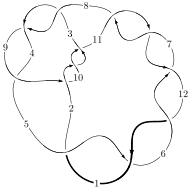
\includegraphics[width=112pt]{../../../GIT/diagram.site/Diagrams/png/2087_12a_1286.png}\\
\ \ \ A knot diagram\footnotemark}&
\allowdisplaybreaks
\textbf{Linearized knot diagam} \\
\cline{2-2}
 &
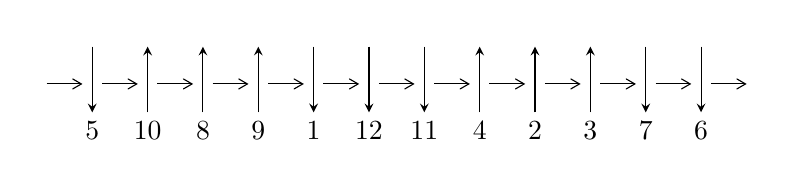
\begin{tikzpicture}[x=20pt, y=17pt]
	% nodes
	\node (C0) at (0, 0) {};
	\node (C1) at (1, 0) {};
	\node (C1U) at (1, +1) {};
	\node (C1D) at (1, -1) {5};

	\node (C2) at (2, 0) {};
	\node (C2U) at (2, +1) {};
	\node (C2D) at (2, -1) {10};

	\node (C3) at (3, 0) {};
	\node (C3U) at (3, +1) {};
	\node (C3D) at (3, -1) {8};

	\node (C4) at (4, 0) {};
	\node (C4U) at (4, +1) {};
	\node (C4D) at (4, -1) {9};

	\node (C5) at (5, 0) {};
	\node (C5U) at (5, +1) {};
	\node (C5D) at (5, -1) {1};

	\node (C6) at (6, 0) {};
	\node (C6U) at (6, +1) {};
	\node (C6D) at (6, -1) {12};

	\node (C7) at (7, 0) {};
	\node (C7U) at (7, +1) {};
	\node (C7D) at (7, -1) {11};

	\node (C8) at (8, 0) {};
	\node (C8U) at (8, +1) {};
	\node (C8D) at (8, -1) {4};

	\node (C9) at (9, 0) {};
	\node (C9U) at (9, +1) {};
	\node (C9D) at (9, -1) {2};

	\node (C10) at (10, 0) {};
	\node (C10U) at (10, +1) {};
	\node (C10D) at (10, -1) {3};

	\node (C11) at (11, 0) {};
	\node (C11U) at (11, +1) {};
	\node (C11D) at (11, -1) {7};

	\node (C12) at (12, 0) {};
	\node (C12U) at (12, +1) {};
	\node (C12D) at (12, -1) {6};
	\node (C13) at (13, 0) {};

	% arrows
	\draw[->,>={angle 60}]
	(C0) edge (C1) (C1) edge (C2) (C2) edge (C3) (C3) edge (C4) (C4) edge (C5) (C5) edge (C6) (C6) edge (C7) (C7) edge (C8) (C8) edge (C9) (C9) edge (C10) (C10) edge (C11) (C11) edge (C12) (C12) edge (C13) ;	\draw[->,>=stealth]
	(C1U) edge (C1D) (C2D) edge (C2U) (C3D) edge (C3U) (C4D) edge (C4U) (C5U) edge (C5D) (C6U) edge (C6D) (C7U) edge (C7D) (C8D) edge (C8U) (C9D) edge (C9U) (C10D) edge (C10U) (C11U) edge (C11D) (C12U) edge (C12D) ;
	\end{tikzpicture} \\
\hhline{~~} \\& 
\textbf{Solving Sequence} \\ \cline{2-2} 
 &
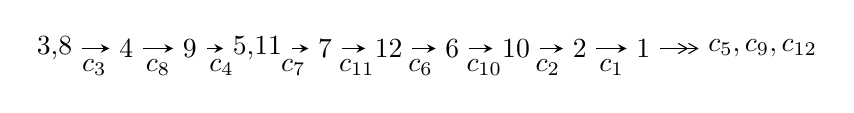
\begin{tikzpicture}[x=23pt, y=7pt]
	% node
	\node (A0) at (-1/8, 0) {3,8};
	\node (A1) at (1, 0) {4};
	\node (A2) at (2, 0) {9};
	\node (A3) at (49/16, 0) {5,11};
	\node (A4) at (33/8, 0) {7};
	\node (A5) at (41/8, 0) {12};
	\node (A6) at (49/8, 0) {6};
	\node (A7) at (57/8, 0) {10};
	\node (A8) at (65/8, 0) {2};
	\node (A9) at (73/8, 0) {1};
	\node (C1) at (1/2, -1) {$c_{3}$};
	\node (C2) at (3/2, -1) {$c_{8}$};
	\node (C3) at (5/2, -1) {$c_{4}$};
	\node (C4) at (29/8, -1) {$c_{7}$};
	\node (C5) at (37/8, -1) {$c_{11}$};
	\node (C6) at (45/8, -1) {$c_{6}$};
	\node (C7) at (53/8, -1) {$c_{10}$};
	\node (C8) at (61/8, -1) {$c_{2}$};
	\node (C9) at (69/8, -1) {$c_{1}$};
	\node (A10) at (11, 0) {$c_{5},c_{9},c_{12}$};

	% edge
	\draw[->,>=stealth]	
	(A0) edge (A1) (A1) edge (A2) (A2) edge (A3) (A3) edge (A4) (A4) edge (A5) (A5) edge (A6) (A6) edge (A7) (A7) edge (A8) (A8) edge (A9) ;
	\draw[->>,>={angle 60}]	
	(A9) edge (A10);
\end{tikzpicture} \\ 

\end{tabular} \\

\footnotetext{
The image of knot diagram is generated by the software ``\textbf{Draw programme}" developed by Andrew Bartholomew(\url{http://www.layer8.co.uk/maths/draw/index.htm\#Running-draw}), where we modified some parts for our purpose(\url{https://github.com/CATsTAILs/LinksPainter}).
}\phantom \\ \newline 
\centering \textbf{Ideals for irreducible components\footnotemark of $X_{\text{par}}$} 
 
\begin{align*}
I^u_{1}&=\langle 
b- u,\;- u^{12}+u^{11}+8 u^{10}-7 u^9-23 u^8+15 u^7+26 u^6-6 u^5-8 u^4-4 u^3+2 u^2+4 a-11 u,\\
\phantom{I^u_{1}}&\phantom{= \langle  }u^{13}- u^{12}-9 u^{11}+8 u^{10}+31 u^9-22 u^8-49 u^7+21 u^6+34 u^5-2 u^4-10 u^3+3 u^2+2 u+1\rangle \\
I^u_{2}&=\langle 
5 u^{13}+u^{12}-28 u^{11}-14 u^{10}+50 u^9+49 u^8-41 u^7-68 u^6+68 u^5+70 u^4-87 u^3-79 u^2+6 b+18 u+30,\\
\phantom{I^u_{2}}&\phantom{= \langle  }17 u^{13}+7 u^{12}+\cdots+24 a+105,\\
\phantom{I^u_{2}}&\phantom{= \langle  }u^{14}- u^{13}-6 u^{12}+4 u^{11}+14 u^{10}-2 u^9-21 u^8-5 u^7+31 u^6- u^5-35 u^4+3 u^3+23 u^2+5 u-8\rangle \\
I^u_{3}&=\langle 
b-1,\;a^2+3,\;u+1\rangle \\
I^u_{4}&=\langle 
b+1,\;a^2+1,\;u-1\rangle \\
I^u_{5}&=\langle 
b-1,\;a,\;u+1\rangle \\
\\
\end{align*}
\raggedright * 5 irreducible components of $\dim_{\mathbb{C}}=0$, with total 32 representations.\\
\footnotetext{All coefficients of polynomials are rational numbers. But the coefficients are sometimes approximated in decimal forms when there is not enough margin.}
\newpage
\renewcommand{\arraystretch}{1}
\centering \section*{I. $I^u_{1}= \langle b- u,\;- u^{12}+u^{11}+\cdots+4 a-11 u,\;u^{13}- u^{12}+\cdots+2 u+1 \rangle$}
\flushleft \textbf{(i) Arc colorings}\\
\begin{tabular}{m{7pt} m{180pt} m{7pt} m{180pt} }
\flushright $a_{3}=$&$\begin{pmatrix}1\\0\end{pmatrix}$ \\
\flushright $a_{8}=$&$\begin{pmatrix}0\\u\end{pmatrix}$ \\
\flushright $a_{4}=$&$\begin{pmatrix}1\\- u^2\end{pmatrix}$ \\
\flushright $a_{9}=$&$\begin{pmatrix}u\\- u^3+u\end{pmatrix}$ \\
\flushright $a_{5}=$&$\begin{pmatrix}- u^2+1\\u^4-2 u^2\end{pmatrix}$ \\
\flushright $a_{11}=$&$\begin{pmatrix}\frac{1}{4} u^{12}-\frac{1}{4} u^{11}+\cdots-\frac{1}{2} u^2+\frac{11}{4} u\\u\end{pmatrix}$ \\
\flushright $a_{7}=$&$\begin{pmatrix}\frac{1}{2} u^{12}-\frac{3}{4} u^{11}+\cdots-\frac{1}{2} u+\frac{1}{4}\\\frac{1}{4} u^{12}-\frac{1}{4} u^{11}+\cdots-\frac{1}{2} u^2+\frac{3}{4} u\end{pmatrix}$ \\
\flushright $a_{12}=$&$\begin{pmatrix}\frac{1}{2} u^{12}-\frac{1}{2} u^{11}+\cdots+2 u+\frac{1}{2}\\\frac{1}{4} u^{12}-\frac{1}{2} u^{11}+\cdots+\frac{3}{4} u+\frac{1}{4}\end{pmatrix}$ \\
\flushright $a_{6}=$&$\begin{pmatrix}-\frac{1}{4} u^{12}+\frac{3}{4} u^{11}+\cdots-2 u^2-\frac{7}{4} u\\\frac{1}{4} u^{12}-\frac{9}{4} u^{10}+\cdots+\frac{1}{4} u+\frac{1}{4}\end{pmatrix}$ \\
\flushright $a_{10}=$&$\begin{pmatrix}\frac{1}{4} u^{12}-\frac{1}{4} u^{11}+\cdots-\frac{1}{2} u^2+\frac{7}{4} u\\u\end{pmatrix}$ \\
\flushright $a_{2}=$&$\begin{pmatrix}\frac{1}{4} u^{11}-\frac{1}{4} u^{10}+\cdots-\frac{1}{2} u+\frac{3}{4}\\u^2\end{pmatrix}$ \\
\flushright $a_{1}=$&$\begin{pmatrix}\frac{1}{4} u^{11}-\frac{1}{4} u^{10}+\cdots-\frac{1}{2} u+\frac{3}{4}\\-\frac{1}{4} u^{11}+\frac{1}{4} u^{10}+\cdots+\frac{1}{2} u+\frac{1}{4}\end{pmatrix}$\\&\end{tabular}
\flushleft \textbf{(ii) Obstruction class $= -1$}\\~\\
\flushleft \textbf{(iii) Cusp Shapes $= \frac{5}{2} u^{12}-\frac{9}{2} u^{11}-21 u^{10}+\frac{75}{2} u^9+\frac{131}{2} u^8-\frac{225}{2} u^7-91 u^6+136 u^5+59 u^4-55 u^3-26 u^2+\frac{45}{2} u+7$}\\~\\
\newpage\renewcommand{\arraystretch}{1}
\flushleft \textbf{(iv) u-Polynomials at the component}\newline \\
\begin{tabular}{m{50pt}|m{274pt}}
Crossings & \hspace{64pt}u-Polynomials at each crossing \\
\hline $$\begin{aligned}c_{1},c_{5},c_{6}\\c_{7},c_{11},c_{12}\end{aligned}$$&$\begin{aligned}
&u^{13}+3 u^{12}+\cdots+12 u+2
\end{aligned}$\\
\hline $$\begin{aligned}c_{2},c_{3},c_{4}\\c_{8},c_{9},c_{10}\end{aligned}$$&$\begin{aligned}
&u^{13}+u^{12}+\cdots+2 u-1
\end{aligned}$\\
\hline
\end{tabular}\\~\\
\newpage\renewcommand{\arraystretch}{1}
\flushleft \textbf{(v) Riley Polynomials at the component}\newline \\
\begin{tabular}{m{50pt}|m{274pt}}
Crossings & \hspace{64pt}Riley Polynomials at each crossing \\
\hline $$\begin{aligned}c_{1},c_{5},c_{6}\\c_{7},c_{11},c_{12}\end{aligned}$$&$\begin{aligned}
&y^{13}+19 y^{12}+\cdots-36 y-4
\end{aligned}$\\
\hline $$\begin{aligned}c_{2},c_{3},c_{4}\\c_{8},c_{9},c_{10}\end{aligned}$$&$\begin{aligned}
&y^{13}-19 y^{12}+\cdots-2 y-1
\end{aligned}$\\
\hline
\end{tabular}\\~\\
\newpage\flushleft \textbf{(vi) Complex Volumes and Cusp Shapes}
$$\begin{array}{c|c|c}  
\text{Solutions to }I^u_{1}& \I (\text{vol} + \sqrt{-1}CS) & \text{Cusp shape}\\
 \hline 
\begin{aligned}
u &= -0.640373 + 0.415565 I \\
a &= -1.25824 + 1.93661 I \\
b &= -0.640373 + 0.415565 I\end{aligned}
 & \phantom{-}15.1852 - 1.4688 I & \phantom{-}6.47409 + 4.73042 I \\ \hline\begin{aligned}
u &= -0.640373 - 0.415565 I \\
a &= -1.25824 - 1.93661 I \\
b &= -0.640373 - 0.415565 I\end{aligned}
 & \phantom{-}15.1852 + 1.4688 I & \phantom{-}6.47409 - 4.73042 I \\ \hline\begin{aligned}
u &= \phantom{-}0.481196 + 0.382474 I \\
a &= \phantom{-}1.09706 + 1.46655 I \\
b &= \phantom{-}0.481196 + 0.382474 I\end{aligned}
 & \phantom{-}4.66648 + 1.38672 I & \phantom{-}6.13236 - 5.06598 I \\ \hline\begin{aligned}
u &= \phantom{-}0.481196 - 0.382474 I \\
a &= \phantom{-}1.09706 - 1.46655 I \\
b &= \phantom{-}0.481196 - 0.382474 I\end{aligned}
 & \phantom{-}4.66648 - 1.38672 I & \phantom{-}6.13236 + 5.06598 I \\ \hline\begin{aligned}
u &= -1.60418\phantom{ +0.000000I} \\
a &= \phantom{-}0.434953\phantom{ +0.000000I} \\
b &= -1.60418\phantom{ +0.000000I}\end{aligned}
 & \phantom{-}10.2165\phantom{ +0.000000I} & \phantom{-}6.80950\phantom{ +0.000000I} \\ \hline\begin{aligned}
u &= \phantom{-}1.61970 + 0.12491 I \\
a &= -0.311845 + 0.455641 I \\
b &= \phantom{-}1.61970 + 0.12491 I\end{aligned}
 & \phantom{-}12.32310 + 4.09027 I & \phantom{-}9.54540 - 4.06441 I \\ \hline\begin{aligned}
u &= \phantom{-}1.61970 - 0.12491 I \\
a &= -0.311845 - 0.455641 I \\
b &= \phantom{-}1.61970 - 0.12491 I\end{aligned}
 & \phantom{-}12.32310 - 4.09027 I & \phantom{-}9.54540 + 4.06441 I \\ \hline\begin{aligned}
u &= -0.187914 + 0.306655 I \\
a &= -0.476417 + 0.917350 I \\
b &= -0.187914 + 0.306655 I\end{aligned}
 & \phantom{-}0.020555 - 0.726577 I & \phantom{-}0.71558 + 9.62371 I \\ \hline\begin{aligned}
u &= -0.187914 - 0.306655 I \\
a &= -0.476417 - 0.917350 I \\
b &= -0.187914 - 0.306655 I\end{aligned}
 & \phantom{-}0.020555 + 0.726577 I & \phantom{-}0.71558 - 9.62371 I \\ \hline\begin{aligned}
u &= -1.65131 + 0.26273 I \\
a &= \phantom{-}0.042681 + 0.832421 I \\
b &= -1.65131 + 0.26273 I\end{aligned}
 & \phantom{-}19.0260 - 7.1684 I & \phantom{-}11.29845 + 3.79891 I\\
 \hline 
 \end{array}$$\newpage$$\begin{array}{c|c|c}  
\text{Solutions to }I^u_{1}& \I (\text{vol} + \sqrt{-1}CS) & \text{Cusp shape}\\
 \hline 
\begin{aligned}
u &= -1.65131 - 0.26273 I \\
a &= \phantom{-}0.042681 - 0.832421 I \\
b &= -1.65131 - 0.26273 I\end{aligned}
 & \phantom{-}19.0260 + 7.1684 I & \phantom{-}11.29845 - 3.79891 I \\ \hline\begin{aligned}
u &= \phantom{-}1.68079 + 0.37590 I \\
a &= \phantom{-}0.189278 + 1.048750 I \\
b &= \phantom{-}1.68079 + 0.37590 I\end{aligned}
 & -8.62649 + 8.95936 I & \phantom{-}11.42936 - 3.31793 I \\ \hline\begin{aligned}
u &= \phantom{-}1.68079 - 0.37590 I \\
a &= \phantom{-}0.189278 - 1.048750 I \\
b &= \phantom{-}1.68079 - 0.37590 I\end{aligned}
 & -8.62649 - 8.95936 I & \phantom{-}11.42936 + 3.31793 I\\
 \hline 
 \end{array}$$\newpage\newpage\renewcommand{\arraystretch}{1}
\centering \section*{II. $I^u_{2}= \langle 5 u^{13}+u^{12}+\cdots+6 b+30,\;17 u^{13}+7 u^{12}+\cdots+24 a+105,\;u^{14}- u^{13}+\cdots+5 u-8 \rangle$}
\flushleft \textbf{(i) Arc colorings}\\
\begin{tabular}{m{7pt} m{180pt} m{7pt} m{180pt} }
\flushright $a_{3}=$&$\begin{pmatrix}1\\0\end{pmatrix}$ \\
\flushright $a_{8}=$&$\begin{pmatrix}0\\u\end{pmatrix}$ \\
\flushright $a_{4}=$&$\begin{pmatrix}1\\- u^2\end{pmatrix}$ \\
\flushright $a_{9}=$&$\begin{pmatrix}u\\- u^3+u\end{pmatrix}$ \\
\flushright $a_{5}=$&$\begin{pmatrix}- u^2+1\\u^4-2 u^2\end{pmatrix}$ \\
\flushright $a_{11}=$&$\begin{pmatrix}-0.708333 u^{13}-0.291667 u^{12}+\cdots-0.125000 u-4.37500\\-\frac{5}{6} u^{13}-\frac{1}{6} u^{12}+\cdots-3 u-5\end{pmatrix}$ \\
\flushright $a_{7}=$&$\begin{pmatrix}-0.208333 u^{13}-0.125000 u^{12}+\cdots-0.458333 u-1.37500\\\frac{1}{2} u^{13}+\frac{1}{6} u^{12}+\cdots+\frac{2}{3} u+3\end{pmatrix}$ \\
\flushright $a_{12}=$&$\begin{pmatrix}-\frac{5}{12} u^{13}-\frac{1}{4} u^{12}+\cdots+\frac{1}{12} u-\frac{11}{4}\\-\frac{5}{3} u^{13}-\frac{1}{3} u^{12}+\cdots-3 u-10\end{pmatrix}$ \\
\flushright $a_{6}=$&$\begin{pmatrix}-0.458333 u^{13}-0.208333 u^{12}+\cdots-0.541667 u-2.12500\\\frac{1}{3} u^{13}+\frac{1}{6} u^{12}+\cdots+\frac{1}{2} u+\frac{7}{3}\end{pmatrix}$ \\
\flushright $a_{10}=$&$\begin{pmatrix}\frac{1}{8} u^{13}-\frac{1}{8} u^{12}+\cdots+\frac{23}{8} u+\frac{5}{8}\\-\frac{5}{6} u^{13}-\frac{1}{6} u^{12}+\cdots-3 u-5\end{pmatrix}$ \\
\flushright $a_{2}=$&$\begin{pmatrix}-0.625000 u^{13}-0.208333 u^{12}+\cdots-1.20833 u-5.12500\\u^{13}+\frac{1}{3} u^{12}+\cdots+\frac{5}{6} u+\frac{23}{3}\end{pmatrix}$ \\
\flushright $a_{1}=$&$\begin{pmatrix}\frac{1}{24} u^{13}+\frac{1}{8} u^{12}+\cdots-\frac{17}{24} u-\frac{1}{8}\\\frac{3}{2} u^{13}+\frac{1}{3} u^{12}+\cdots+\frac{11}{6} u+\frac{31}{3}\end{pmatrix}$\\&\end{tabular}
\flushleft \textbf{(ii) Obstruction class $= -1$}\\~\\
\flushleft \textbf{(iii) Cusp Shapes $= -\frac{26}{3} u^{13}-\frac{8}{3} u^{12}+50 u^{11}+28 u^{10}-90 u^9-92 u^8+\frac{208}{3} u^7+\frac{392}{3} u^6-\frac{344}{3} u^5-136 u^4+\frac{446}{3} u^3+146 u^2-\frac{46}{3} u-\frac{158}{3}$}\\~\\
\newpage\renewcommand{\arraystretch}{1}
\flushleft \textbf{(iv) u-Polynomials at the component}\newline \\
\begin{tabular}{m{50pt}|m{274pt}}
Crossings & \hspace{64pt}u-Polynomials at each crossing \\
\hline $$\begin{aligned}c_{1},c_{5},c_{6}\\c_{7},c_{11},c_{12}\end{aligned}$$&$\begin{aligned}
&(u^7- u^6+6 u^5-5 u^4+10 u^3-6 u^2+4 u-1)^2
\end{aligned}$\\
\hline $$\begin{aligned}c_{2},c_{3},c_{4}\\c_{8},c_{9},c_{10}\end{aligned}$$&$\begin{aligned}
&u^{14}+u^{13}+\cdots-5 u-8
\end{aligned}$\\
\hline
\end{tabular}\\~\\
\newpage\renewcommand{\arraystretch}{1}
\flushleft \textbf{(v) Riley Polynomials at the component}\newline \\
\begin{tabular}{m{50pt}|m{274pt}}
Crossings & \hspace{64pt}Riley Polynomials at each crossing \\
\hline $$\begin{aligned}c_{1},c_{5},c_{6}\\c_{7},c_{11},c_{12}\end{aligned}$$&$\begin{aligned}
&(y^7+11 y^6+46 y^5+91 y^4+86 y^3+34 y^2+4 y-1)^2
\end{aligned}$\\
\hline $$\begin{aligned}c_{2},c_{3},c_{4}\\c_{8},c_{9},c_{10}\end{aligned}$$&$\begin{aligned}
&y^{14}-13 y^{13}+\cdots-393 y+64
\end{aligned}$\\
\hline
\end{tabular}\\~\\
\newpage\flushleft \textbf{(vi) Complex Volumes and Cusp Shapes}
$$\begin{array}{c|c|c}  
\text{Solutions to }I^u_{2}& \I (\text{vol} + \sqrt{-1}CS) & \text{Cusp shape}\\
 \hline 
\begin{aligned}
u &= \phantom{-}0.648339 + 0.868507 I \\
a &= -0.946848 - 0.814097 I \\
b &= -1.49879 - 0.07472 I\end{aligned}
 & \phantom{-}11.28970 + 2.92126 I & \phantom{-}9.79653 - 2.94858 I \\ \hline\begin{aligned}
u &= \phantom{-}0.648339 - 0.868507 I \\
a &= -0.946848 + 0.814097 I \\
b &= -1.49879 + 0.07472 I\end{aligned}
 & \phantom{-}11.28970 - 2.92126 I & \phantom{-}9.79653 + 2.94858 I \\ \hline\begin{aligned}
u &= -1.15470\phantom{ +0.000000I} \\
a &= -0.288944\phantom{ +0.000000I} \\
b &= \phantom{-}0.577082\phantom{ +0.000000I}\end{aligned}
 & \phantom{-}2.54463\phantom{ +0.000000I} & -1.98880\phantom{ +0.000000I} \\ \hline\begin{aligned}
u &= -0.613438 + 0.507408 I \\
a &= \phantom{-}0.322269 - 0.816953 I \\
b &= \phantom{-}1.290190 - 0.016333 I\end{aligned}
 & \phantom{-}4.55769 - 1.83261 I & \phantom{-}8.22558 + 5.43914 I \\ \hline\begin{aligned}
u &= -0.613438 - 0.507408 I \\
a &= \phantom{-}0.322269 + 0.816953 I \\
b &= \phantom{-}1.290190 + 0.016333 I\end{aligned}
 & \phantom{-}4.55769 + 1.83261 I & \phantom{-}8.22558 - 5.43914 I \\ \hline\begin{aligned}
u &= -0.674237 + 1.068950 I \\
a &= \phantom{-}1.21462 - 0.78780 I \\
b &= \phantom{-}1.63675 - 0.11855 I\end{aligned}
 & -16.2972 - 3.4867 I & \phantom{-}9.97231 + 2.18600 I \\ \hline\begin{aligned}
u &= -0.674237 - 1.068950 I \\
a &= \phantom{-}1.21462 + 0.78780 I \\
b &= \phantom{-}1.63675 + 0.11855 I\end{aligned}
 & -16.2972 + 3.4867 I & \phantom{-}9.97231 - 2.18600 I \\ \hline\begin{aligned}
u &= \phantom{-}1.290190 + 0.016333 I \\
a &= \phantom{-}0.161518 - 0.517219 I \\
b &= -0.613438 - 0.507408 I\end{aligned}
 & \phantom{-}4.55769 + 1.83261 I & \phantom{-}8.22558 - 5.43914 I \\ \hline\begin{aligned}
u &= \phantom{-}1.290190 - 0.016333 I \\
a &= \phantom{-}0.161518 + 0.517219 I \\
b &= -0.613438 + 0.507408 I\end{aligned}
 & \phantom{-}4.55769 - 1.83261 I & \phantom{-}8.22558 + 5.43914 I \\ \hline\begin{aligned}
u &= \phantom{-}0.577082\phantom{ +0.000000I} \\
a &= \phantom{-}0.578156\phantom{ +0.000000I} \\
b &= -1.15470\phantom{ +0.000000I}\end{aligned}
 & \phantom{-}2.54463\phantom{ +0.000000I} & -1.98880\phantom{ +0.000000I}\\
 \hline 
 \end{array}$$\newpage$$\begin{array}{c|c|c}  
\text{Solutions to }I^u_{2}& \I (\text{vol} + \sqrt{-1}CS) & \text{Cusp shape}\\
 \hline 
\begin{aligned}
u &= -1.49879 + 0.07472 I \\
a &= -0.017211 - 0.901687 I \\
b &= \phantom{-}0.648339 - 0.868507 I\end{aligned}
 & \phantom{-}11.28970 - 2.92126 I & \phantom{-}9.79653 + 2.94858 I \\ \hline\begin{aligned}
u &= -1.49879 - 0.07472 I \\
a &= -0.017211 + 0.901687 I \\
b &= \phantom{-}0.648339 + 0.868507 I\end{aligned}
 & \phantom{-}11.28970 + 2.92126 I & \phantom{-}9.79653 - 2.94858 I \\ \hline\begin{aligned}
u &= \phantom{-}1.63675 + 0.11855 I \\
a &= -0.066458 - 1.112970 I \\
b &= -0.674237 - 1.068950 I\end{aligned}
 & -16.2972 + 3.4867 I & \phantom{-}9.97231 - 2.18600 I \\ \hline\begin{aligned}
u &= \phantom{-}1.63675 - 0.11855 I \\
a &= -0.066458 + 1.112970 I \\
b &= -0.674237 + 1.068950 I\end{aligned}
 & -16.2972 - 3.4867 I & \phantom{-}9.97231 + 2.18600 I\\
 \hline 
 \end{array}$$\newpage\newpage\renewcommand{\arraystretch}{1}
\centering \section*{III. $I^u_{3}= \langle b-1,\;a^2+3,\;u+1 \rangle$}
\flushleft \textbf{(i) Arc colorings}\\
\begin{tabular}{m{7pt} m{180pt} m{7pt} m{180pt} }
\flushright $a_{3}=$&$\begin{pmatrix}1\\0\end{pmatrix}$ \\
\flushright $a_{8}=$&$\begin{pmatrix}0\\-1\end{pmatrix}$ \\
\flushright $a_{4}=$&$\begin{pmatrix}1\\-1\end{pmatrix}$ \\
\flushright $a_{9}=$&$\begin{pmatrix}-1\\0\end{pmatrix}$ \\
\flushright $a_{5}=$&$\begin{pmatrix}0\\-1\end{pmatrix}$ \\
\flushright $a_{11}=$&$\begin{pmatrix}a\\1\end{pmatrix}$ \\
\flushright $a_{7}=$&$\begin{pmatrix}3\\- a-1\end{pmatrix}$ \\
\flushright $a_{12}=$&$\begin{pmatrix}-2 a\\a-2\end{pmatrix}$ \\
\flushright $a_{6}=$&$\begin{pmatrix}-3\\a+2\end{pmatrix}$ \\
\flushright $a_{10}=$&$\begin{pmatrix}a-1\\1\end{pmatrix}$ \\
\flushright $a_{2}=$&$\begin{pmatrix}a\\1\end{pmatrix}$ \\
\flushright $a_{1}=$&$\begin{pmatrix}a\\- a+1\end{pmatrix}$\\&\end{tabular}
\flushleft \textbf{(ii) Obstruction class $= 1$}\\~\\
\flushleft \textbf{(iii) Cusp Shapes $= 12$}\\~\\
\newpage\renewcommand{\arraystretch}{1}
\flushleft \textbf{(iv) u-Polynomials at the component}\newline \\
\begin{tabular}{m{50pt}|m{274pt}}
Crossings & \hspace{64pt}u-Polynomials at each crossing \\
\hline $$\begin{aligned}c_{1},c_{5},c_{6}\\c_{7},c_{11},c_{12}\end{aligned}$$&$\begin{aligned}
&u^2+3
\end{aligned}$\\
\hline $$\begin{aligned}c_{2},c_{8}\end{aligned}$$&$\begin{aligned}
&(u-1)^2
\end{aligned}$\\
\hline $$\begin{aligned}c_{3},c_{4},c_{9}\\c_{10}\end{aligned}$$&$\begin{aligned}
&(u+1)^2
\end{aligned}$\\
\hline
\end{tabular}\\~\\
\newpage\renewcommand{\arraystretch}{1}
\flushleft \textbf{(v) Riley Polynomials at the component}\newline \\
\begin{tabular}{m{50pt}|m{274pt}}
Crossings & \hspace{64pt}Riley Polynomials at each crossing \\
\hline $$\begin{aligned}c_{1},c_{5},c_{6}\\c_{7},c_{11},c_{12}\end{aligned}$$&$\begin{aligned}
&(y+3)^2
\end{aligned}$\\
\hline $$\begin{aligned}c_{2},c_{3},c_{4}\\c_{8},c_{9},c_{10}\end{aligned}$$&$\begin{aligned}
&(y-1)^2
\end{aligned}$\\
\hline
\end{tabular}\\~\\
\newpage\flushleft \textbf{(vi) Complex Volumes and Cusp Shapes}
$$\begin{array}{c|c|c}  
\text{Solutions to }I^u_{3}& \I (\text{vol} + \sqrt{-1}CS) & \text{Cusp shape}\\
 \hline 
\begin{aligned}
u &= -1.00000\phantom{ +0.000000I} \\
a &= \phantom{-0.000000 -}1.73205 I \\
b &= \phantom{-}1.00000\phantom{ +0.000000I}\end{aligned}
 & \phantom{-}16.4493\phantom{ +0.000000I} & \phantom{-}12.0000\phantom{ +0.000000I} \\ \hline\begin{aligned}
u &= -1.00000\phantom{ +0.000000I} \\
a &= \phantom{-0.000000 } -1.73205 I \\
b &= \phantom{-}1.00000\phantom{ +0.000000I}\end{aligned}
 & \phantom{-}16.4493\phantom{ +0.000000I} & \phantom{-}12.0000\phantom{ +0.000000I}\\
 \hline 
 \end{array}$$\newpage\newpage\renewcommand{\arraystretch}{1}
\centering \section*{IV. $I^u_{4}= \langle b+1,\;a^2+1,\;u-1 \rangle$}
\flushleft \textbf{(i) Arc colorings}\\
\begin{tabular}{m{7pt} m{180pt} m{7pt} m{180pt} }
\flushright $a_{3}=$&$\begin{pmatrix}1\\0\end{pmatrix}$ \\
\flushright $a_{8}=$&$\begin{pmatrix}0\\1\end{pmatrix}$ \\
\flushright $a_{4}=$&$\begin{pmatrix}1\\-1\end{pmatrix}$ \\
\flushright $a_{9}=$&$\begin{pmatrix}1\\0\end{pmatrix}$ \\
\flushright $a_{5}=$&$\begin{pmatrix}0\\-1\end{pmatrix}$ \\
\flushright $a_{11}=$&$\begin{pmatrix}a\\-1\end{pmatrix}$ \\
\flushright $a_{7}=$&$\begin{pmatrix}-1\\- a+1\end{pmatrix}$ \\
\flushright $a_{12}=$&$\begin{pmatrix}0\\a\end{pmatrix}$ \\
\flushright $a_{6}=$&$\begin{pmatrix}-1\\- a\end{pmatrix}$ \\
\flushright $a_{10}=$&$\begin{pmatrix}a+1\\-1\end{pmatrix}$ \\
\flushright $a_{2}=$&$\begin{pmatrix}- a\\1\end{pmatrix}$ \\
\flushright $a_{1}=$&$\begin{pmatrix}- a\\a+1\end{pmatrix}$\\&\end{tabular}
\flushleft \textbf{(ii) Obstruction class $= 1$}\\~\\
\flushleft \textbf{(iii) Cusp Shapes $= 12$}\\~\\
\newpage\renewcommand{\arraystretch}{1}
\flushleft \textbf{(iv) u-Polynomials at the component}\newline \\
\begin{tabular}{m{50pt}|m{274pt}}
Crossings & \hspace{64pt}u-Polynomials at each crossing \\
\hline $$\begin{aligned}c_{1},c_{5},c_{6}\\c_{7},c_{11},c_{12}\end{aligned}$$&$\begin{aligned}
&u^2+1
\end{aligned}$\\
\hline $$\begin{aligned}c_{2},c_{8}\end{aligned}$$&$\begin{aligned}
&(u+1)^2
\end{aligned}$\\
\hline $$\begin{aligned}c_{3},c_{4},c_{9}\\c_{10}\end{aligned}$$&$\begin{aligned}
&(u-1)^2
\end{aligned}$\\
\hline
\end{tabular}\\~\\
\newpage\renewcommand{\arraystretch}{1}
\flushleft \textbf{(v) Riley Polynomials at the component}\newline \\
\begin{tabular}{m{50pt}|m{274pt}}
Crossings & \hspace{64pt}Riley Polynomials at each crossing \\
\hline $$\begin{aligned}c_{1},c_{5},c_{6}\\c_{7},c_{11},c_{12}\end{aligned}$$&$\begin{aligned}
&(y+1)^2
\end{aligned}$\\
\hline $$\begin{aligned}c_{2},c_{3},c_{4}\\c_{8},c_{9},c_{10}\end{aligned}$$&$\begin{aligned}
&(y-1)^2
\end{aligned}$\\
\hline
\end{tabular}\\~\\
\newpage\flushleft \textbf{(vi) Complex Volumes and Cusp Shapes}
$$\begin{array}{c|c|c}  
\text{Solutions to }I^u_{4}& \I (\text{vol} + \sqrt{-1}CS) & \text{Cusp shape}\\
 \hline 
\begin{aligned}
u &= \phantom{-}1.00000\phantom{ +0.000000I} \\
a &= \phantom{-0.000000 -}1.000000 I \\
b &= -1.00000\phantom{ +0.000000I}\end{aligned}
 & \phantom{-}6.57974\phantom{ +0.000000I} & \phantom{-}12.0000\phantom{ +0.000000I} \\ \hline\begin{aligned}
u &= \phantom{-}1.00000\phantom{ +0.000000I} \\
a &= \phantom{-0.000000 } -1.000000 I \\
b &= -1.00000\phantom{ +0.000000I}\end{aligned}
 & \phantom{-}6.57974\phantom{ +0.000000I} & \phantom{-}12.0000\phantom{ +0.000000I}\\
 \hline 
 \end{array}$$\newpage\newpage\renewcommand{\arraystretch}{1}
\centering \section*{V. $I^u_{5}= \langle b-1,\;a,\;u+1 \rangle$}
\flushleft \textbf{(i) Arc colorings}\\
\begin{tabular}{m{7pt} m{180pt} m{7pt} m{180pt} }
\flushright $a_{3}=$&$\begin{pmatrix}1\\0\end{pmatrix}$ \\
\flushright $a_{8}=$&$\begin{pmatrix}0\\-1\end{pmatrix}$ \\
\flushright $a_{4}=$&$\begin{pmatrix}1\\-1\end{pmatrix}$ \\
\flushright $a_{9}=$&$\begin{pmatrix}-1\\0\end{pmatrix}$ \\
\flushright $a_{5}=$&$\begin{pmatrix}0\\-1\end{pmatrix}$ \\
\flushright $a_{11}=$&$\begin{pmatrix}0\\1\end{pmatrix}$ \\
\flushright $a_{7}=$&$\begin{pmatrix}0\\-1\end{pmatrix}$ \\
\flushright $a_{12}=$&$\begin{pmatrix}0\\1\end{pmatrix}$ \\
\flushright $a_{6}=$&$\begin{pmatrix}0\\-1\end{pmatrix}$ \\
\flushright $a_{10}=$&$\begin{pmatrix}-1\\1\end{pmatrix}$ \\
\flushright $a_{2}=$&$\begin{pmatrix}0\\1\end{pmatrix}$ \\
\flushright $a_{1}=$&$\begin{pmatrix}0\\1\end{pmatrix}$\\&\end{tabular}
\flushleft \textbf{(ii) Obstruction class $= 1$}\\~\\
\flushleft \textbf{(iii) Cusp Shapes $= 12$}\\~\\
\newpage\renewcommand{\arraystretch}{1}
\flushleft \textbf{(iv) u-Polynomials at the component}\newline \\
\begin{tabular}{m{50pt}|m{274pt}}
Crossings & \hspace{64pt}u-Polynomials at each crossing \\
\hline $$\begin{aligned}c_{1},c_{5},c_{6}\\c_{7},c_{11},c_{12}\end{aligned}$$&$\begin{aligned}
&u
\end{aligned}$\\
\hline $$\begin{aligned}c_{2},c_{8}\end{aligned}$$&$\begin{aligned}
&u-1
\end{aligned}$\\
\hline $$\begin{aligned}c_{3},c_{4},c_{9}\\c_{10}\end{aligned}$$&$\begin{aligned}
&u+1
\end{aligned}$\\
\hline
\end{tabular}\\~\\
\newpage\renewcommand{\arraystretch}{1}
\flushleft \textbf{(v) Riley Polynomials at the component}\newline \\
\begin{tabular}{m{50pt}|m{274pt}}
Crossings & \hspace{64pt}Riley Polynomials at each crossing \\
\hline $$\begin{aligned}c_{1},c_{5},c_{6}\\c_{7},c_{11},c_{12}\end{aligned}$$&$\begin{aligned}
&y
\end{aligned}$\\
\hline $$\begin{aligned}c_{2},c_{3},c_{4}\\c_{8},c_{9},c_{10}\end{aligned}$$&$\begin{aligned}
&y-1
\end{aligned}$\\
\hline
\end{tabular}\\~\\
\newpage\flushleft \textbf{(vi) Complex Volumes and Cusp Shapes}
$$\begin{array}{c|c|c}  
\text{Solutions to }I^u_{5}& \I (\text{vol} + \sqrt{-1}CS) & \text{Cusp shape}\\
 \hline 
\begin{aligned}
u &= -1.00000\phantom{ +0.000000I} \\
a &= \phantom{-0.000000 } 0 \\
b &= \phantom{-}1.00000\phantom{ +0.000000I}\end{aligned}
 & \phantom{-}3.28987\phantom{ +0.000000I} & \phantom{-}12.0000\phantom{ +0.000000I}\\
 \hline 
 \end{array}$$\newpage
\newpage\renewcommand{\arraystretch}{1}
\centering \section*{ VI. u-Polynomials}
\begin{tabular}{m{50pt}|m{274pt}}
Crossings & \hspace{64pt}u-Polynomials at each crossing \\
\hline $$\begin{aligned}c_{1},c_{5},c_{6}\\c_{7},c_{11},c_{12}\end{aligned}$$&$\begin{aligned}
&u(u^2+1)(u^2+3)(u^7- u^6+6 u^5-5 u^4+10 u^3-6 u^2+4 u-1)^2\\
&\cdot(u^{13}+3 u^{12}+\cdots+12 u+2)
\end{aligned}$\\
\hline $$\begin{aligned}c_{2},c_{8}\end{aligned}$$&$\begin{aligned}
&((u-1)^3)(u+1)^2(u^{13}+u^{12}+\cdots+2 u-1)(u^{14}+u^{13}+\cdots-5 u-8)
\end{aligned}$\\
\hline $$\begin{aligned}c_{3},c_{4},c_{9}\\c_{10}\end{aligned}$$&$\begin{aligned}
&((u-1)^2)(u+1)^3(u^{13}+u^{12}+\cdots+2 u-1)(u^{14}+u^{13}+\cdots-5 u-8)
\end{aligned}$\\
\hline
\end{tabular}\newpage\renewcommand{\arraystretch}{1}
\centering \section*{ VII. Riley Polynomials}
\begin{tabular}{m{50pt}|m{274pt}}
Crossings & \hspace{64pt}Riley Polynomials at each crossing \\
\hline $$\begin{aligned}c_{1},c_{5},c_{6}\\c_{7},c_{11},c_{12}\end{aligned}$$&$\begin{aligned}
&y(y+1)^2(y+3)^2\\
&\cdot(y^7+11 y^6+46 y^5+91 y^4+86 y^3+34 y^2+4 y-1)^2\\
&\cdot(y^{13}+19 y^{12}+\cdots-36 y-4)
\end{aligned}$\\
\hline $$\begin{aligned}c_{2},c_{3},c_{4}\\c_{8},c_{9},c_{10}\end{aligned}$$&$\begin{aligned}
&((y-1)^5)(y^{13}-19 y^{12}+\cdots-2 y-1)(y^{14}-13 y^{13}+\cdots-393 y+64)
\end{aligned}$\\
\hline
\end{tabular}
\vskip 2pc
\end{document}